\section{Introduction}

There is an almost ubiquitous growing demand for mobile and wireless data, with consumers demanding faster speeds and better quality connections in more places. Consequently 4G is now being rolled out in the UK and US and with 5G being planned for 2020 and beyond \cite{Dahlman2014}.  

However, there is constrained amount of frequencies over which to transmit this information; and demand for frequencies that provide sufficient bandwidth, good range and in-building penetration is high.

Not all spectrum is used in all places and at all times, and judicious spectrum management, by developing approaches to use white spaces where they occur, would likely be beneficial.

Broadly, access to spectrum is managed in two, complementary ways, namely through licensed and licence exempt access. Licensing authorises a particular user (or users) to access a specific frequency band. Licence exemption allows any user to access a band provided they meet certain technical requirements intended to limit the impact of interference on other spectrum users.

A licence exempt approach might be particularly suitable for managing access to white spaces. Devices seeking to access white spaces need a robust mechanism for learning of the frequencies that can be used at a particular time and location. One approach is to refer to a database, which maps the location of white spaces based on knowledge of existing spectrum users. An alternative approach is for devices to detect white spaces by monitoring spectrum use. 

The advantages of spectrum monitoring \cite{akan2009cognitive} over maintaining a database of space-frequency data are the ability of networks to make use of low-cost low-power devices, only capable of making local (as opposed to national) communications, keeping the cost of the network low and  opportunistic channel usage for bursty traffic, reducing channel collisions in dense networks.

The realisation of any Cognitive Radio standard (such as IEEE 802.22 \cite{stevenson2009ieee}), requires the co-existence of primary (e.g. TV users) and secondary (everybody else who wants to use TVWS spectrum) users of the frequency spectrum to ensure proper interference mitigation and appropriate network behaviour. We note, that whereas TVWS bands are an initial step towards dynamic spectrum access, the principles and approaches we describe are applicable to other frequency bands - in particular it makes ultra-wideband spectrum sensing possible.

The challenges of this technology are that Cognitive Radios (CRs) must sense whether spectrum is available, and must be able to detect very weak primary user signals. Furthermore they must sense over a wide bandwidth (due to the amount of TVWS spectrum proposed), which challenges traditional Nyquist sampling techniques, because the sampling rates required are not technically feasible with current RF or Analogue-to-Digital conversion technology.

Due to the inherent sparsity of spectral utilisation, Compressive Sensing (CS) \cite{Candes2006} is an appropriate formalism within which to tackle this problem. CS has recently emerged as a new sampling paradigm allowing images to be taken from a single pixel camera for example. Applying this to wireless communication, we are able to reconstruct sparse signals at sampling rates below what would be required by Nyquist theory, for example the works \cite{mishali2010theory}, \cite{Mishali2010a}, \cite{Mishali2009}, \cite{Mishali2011}, and \cite{tropp2010beyond} detail how this sampling can be achieved. 

However, even with CS, spectrum sensing from a single machine will be costly as the proposed TVWS band will be over a large frequency range (for instance in the UK the proposed TVWS band is from 470 MHz to 790 MHz, requiring traditional sampling rates of \textasciitilde 600 MHz). CS at a single sensor would still require high sampling rates. In this report we propose a distributed model, which allows a sensing budget at each node far below what is required by centralised CS.

\section{Wideband Spectrum Sensing}
This section presents a new method of sensing sparse signals, and its application to the problem of sensing over wideband spectra in Cognitive Radios. Initially we introduce Classical Sensing and then give an overview of both Compressive Sensing and Group Testing. Finally, we discuss some sub-Nyquist sampling techniques.

\begin{figure*}[h]
\centering
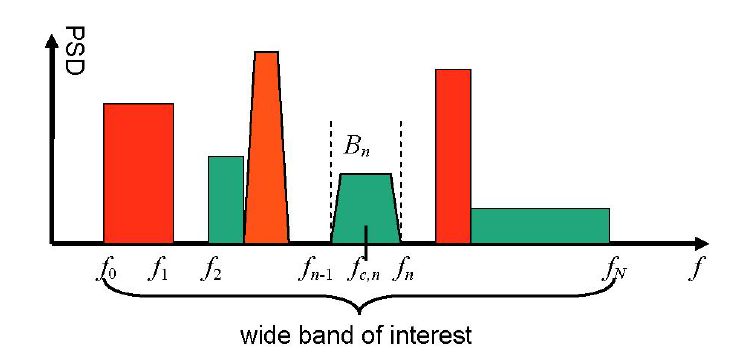
\includegraphics[height = 7 cm]{bands.png}
\caption{A digram of the Spectrum Sensing model \cite{Tian}}
\label{widebandspectra}
\end{figure*}

\subsection{Compressed Sensing}

Compressive sensing is a modern signal acquisition technique in which randomness is used as an effective sensing strategy for classes of signals typically encountered in practice.

Informally, CS posits that for \(k\)-sparse signals \(\in \re^{n}\) - signals with \(k\) non-zero amplitudes at unknown locations) - \(k\log{n}\) measurements are sufficient to exactly reconstruct the signal. In other words we can sample at the information rate, without information loss.

For TVWS signals, this reasoning can be inverted: signals with very large bandwidth - but with a sparse spectrum - can be sampled randomly in time at rates below below those thought sufficient by the Nyquist theorem.

This work has been extended to cases where the signal isn't exactly sparse, and where the measurements are imperfect.

The central idea of CS is that randomness is an effective sensing strategy. We require that sensing vectors satisfy two technical conditions (described in detail below): an Isotropy property, which means that components of the sensing vectors have unit variance and are uncorrelated, and an Incoherence property, which means that sensing vectors are almost orthogonal. These conditions are summed up in the Restricted Isometry Property.

Once the set of measurements have been taken, the signal may be reconstructed from a simple linear program.

In practice many signals encountered 'in the wild' can be fully specified by much fewer bits than required by the Nyquist sampling theorem. This is either a natural property of the signals, for example images have large areas of similar pixels, or as a conscious design choice, for example training sequences in communication transmissions. These signals are not statistically white, and so these signals may be compressed (to save on storage). For example, lossy image compression algorithms can reduce the size of a stored image to about 1\% of the size required by Nyquist sampling. 

Whilst this vein of research has been extraordinarily successful, it poses the question: if the reconstruction algorithm is able to reconstruct the signal from this compressed representation, why collect all the data in the first place, when most of the information can be thrown away? Is it possible to directly measure the part that will not end up being thrown away?

Compressed Sensing answers these questions, by way of providing an alternative signal acquisition method to the Nyquist theorem. Specifically, situations are considered where fewer samples are collected than traditional sensing schemes. 

That is, in contrast to Nyquist sampling, Compressive Sensing is a method of measuring the informative parts of a signal directly without acquiring unessential information at the same time. 

Signals which are compressible, are signals whose information content is smaller than the ambient dimension they are acquired in. Such signals have representations in which they are sparse (i.e. the most of the co-efficients in that representation are zero, or close to zero). For example, 

\begin{enumerate}
\item  A sine wave at frequency \(\omega\) is defined as a single spike in the frequency domain yet has an infinite support in the time domain
\item An image will have values for every pixel, yet the wavelet decomposition of the image will typically only have a few non-zero coefficients
\end{enumerate} 

We may not be able to directly obtain those coefficients, as we may not posses an appropriate measuring device or one may not exist, or there is considerable uncertainty about where the non-zero coefficients are. Yet we still are able to measure correlations between the signal and some waveforms \(\phi_{k}\) i.e. 
%
\begin{equation}
y_{k} = \left\langle f \text{,} \phi_{k} \right\rangle \text{ } k = 1 \ldots m
\end{equation}
%
for \( f \in \mathbb{R}^n \) expanded in an orthonormal basis \( \psi \) s.t.
%
\begin{equation}
f(t) = \sum_{i = 1}^n x_{i}\psi_{i}(t) 
\end{equation}
%
where the \(x_{i} \) are the coefficient sequence of f. 

%An example of a practical Compressive Sensing system is the single-pixel camera at Rice University \cite{Duarte2008}. Typical camera devices obtain pixel samples by exposing a bank of photon detectors (one for each pixel) to the incident light field. This data is the processed into an image.

%The single pixel camera takes pictures by first directing the incoming light field onto an array of tiny mirrors (one for each pixel). Each mirror can be either be oriented towards a single photon detector, or oriented away from the detector. In this setup, a measurement is taken as the sum of all the incident light beams. Afterwards, the mirrors are flipped to a new random configuration, and another measurement is taken. This process is repeated, until enough information has been collected to reconstruct the image. Figure \ref{singlepixelcamera} shows the operation of the single pixel camera.

%\begin{figure*}[h]
%\centering
%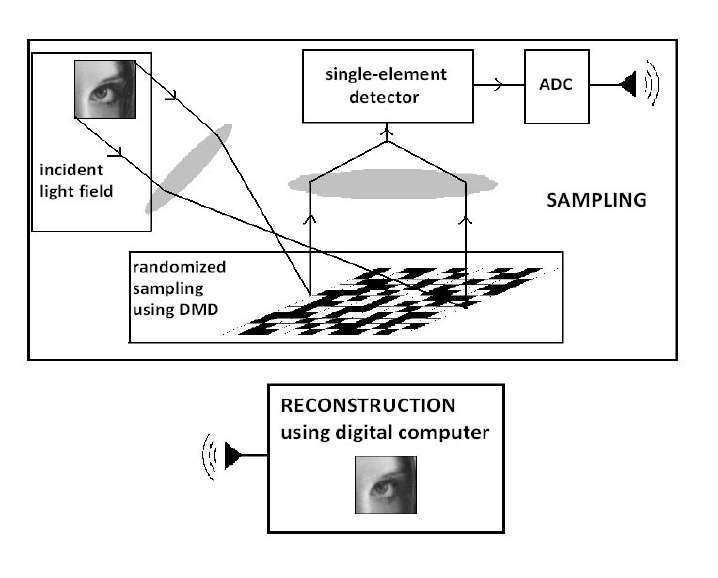
\includegraphics[height = 7 cm]{singlepixel.png}
%\caption{The operation of the single pixel camera at Rice University \cite{singlepixelimaging}}
%\label{singlepixelcamera}
%\end{figure*}

%Compressive Sensing works best if the \(x_{i}\) are compressible (i.e. they are distributed according to a power law), and the error \(\|x - x_{s}\|\) is small.

%In Compressive Sensing measurements are taken is an incoherent basis, as opposed to the basis of the original signal. 

Given that we know a basis in which our signal is sparse, \(\phi\), how do we choose \(\psi\), so that we can accomplish this sensing task? In classical sensing, we choose \(\psi_k\) to be the set of \( T_s \)-spaced delta functions (or equivalently the set of \( 1/T_s \) spaced delta functions in the frequency domain). A simple set of \(\psi_k\) would be to choose a (random) subset of the delta functions above.

In general, we seek waveforms in which the signals' representation would be dense.

\begin{defn}
A pair of bases is said to be incoherent if the largest projection of two elements between the sensing (\(\psi\)) and representation (\(\phi\)) basis  is in the set \( [1 , \sqrt{n}] \), where \( n \) is the dimension of the signal. 
\end{defn}

The coherence of a set of bases is denoted by \(\mu\).

This implies that sensing with incoherent systems is good (in the sine wave example above it would be better to sample randomly in the time domain as opposed to the frequency domain), and efficient mechanisms ought to acquire correlations with random waveforms (e.g. white noise).

\textbf{Theorem} \cite{Candes2006}
Fix a signal f \(\in \mathbb{R}^n\) with a sparse coefficient basis, \(x_{i}\) in \(\phi\). Then a reconstruction from \(m\) random measurements in \(\psi\) is possible with probability \(1 - \delta\) if: 

\begin{equation}
m \geq C \mu^2(\phi, \psi) S \log\left(\frac{n}{\delta}\right)
\end{equation}
\label{minsamples}

where \( \mu(\phi, \psi)\) is the coherence of the two bases, and \(S\) is the number of non-zero entries on the support of the signal.

Once we have obtained the measurements \(m\), we need to reconstruct the signal. 

To recover a sparse vector, we must make sure that the vectors are not in the null space of the sensing matrix (otherwise there would be no hope of recovery). We also require that any subset of \(S\) columns taken from the measurement matrix be nearly orthogonal w.r.t sparse vectors: i.e. all pairwise distances between S-sparse vecotrs be well preserved in the measurement space.

This can be summed up in the following inequality (Restricted Isometry Property) \cite{Emma}:

\begin{equation}
\left(1-\delta\right)\vectornorm{x}_{l_2}^2 \leq \vectornorm{Ax}_{l_2}^2 \leq \left(1+\delta\right) \vectornorm{x}_{l_2}^2
\end{equation}
\label{RIP}

We are also in a position to evaluate the meaning of the constant \(\mu\) in \ref{minsamples}. We are considering sampling within orthonormal systems (for example, Time and Frequency):
%
\begin{equation}
A*A = nI
\end{equation}
\label{orthonormal}
%
so that each row or column has \(l_2\) norm equal to \(sqrt{n}\). \(A\) is any matrix satisfying this property (examples include the Fourier matrix and the Dirac matrix). Thus \(\mu\) must be in the set \(\left[1, \sqrt{n}\right]\). \(\mu\) then, is a measure of how concentrated the rows of our measurement matrix is - i.e. how much information is spread across each vector. If \(\mu = 1\) then the rows are 'flat' -  and we need relatively fewer samples to reconstruct an S-sparse signal (i.e. each sample provides the same amount of information). However, if the rows contain all non-zero entries except for a single component, then \(\mu^2 = n\) and we will need to observe all components to determine the non-zero one (i.e. we have no guarantees of recovery from limited samples) \cite{Candes2007}. 

Noting that the measurements we take are projections from our orthonormal system (from example time) onto a sparsifying basis (i.e. frequency) we can see that:

\begin{equation}
\mu = max_{k,j} |\langle \phi_k, \psi_j \rangle |
\end{equation}
\label {mudef}
 
So we need to choose a sensing basis, where the vectors will be 'spread out', and the degree of spreading is characterised by \(\mu\).

The correct functional to minimise would be:

\begin{equation}
min\|\tilde{x}\|_{l_{0}} \text{ subject to } y_{k} = \langle \phi_{k} \text{,} \psi x^* \rangle \text{   } \forall k \in M \subset [1 \ldots n]
\end{equation}
\label{programl0}

where 

\begin{equation}
|| s ||_0 = |s|
\end{equation}

However, this norm is not convex and so minimising it is an NP-hard optimisation problem. As we are seeking sparse solutions the \(l_1\)-norm will suffice \cite{Donoho2006a}. This is because all vectors in a random \(k\)-dimensional subspace of an \(n\)-dimensional space are approximately Gaussian (in the sense that the components are distributed according to an approximate normal distribution). Such vectors have roughly equivalent norms, and so any solution to the \(l_1\) minimisation problem will be the same solution to the \(l_0\) minimisation problem for sufficiently sparse signals.

Thus the role of \(l_{1}\) minimisation is to decompress the data. There are many ways to perform this operation: some popular methods are basis pursuit \cite{Chen1998} and Greedy approaches such as Orthogonal Matching Pursuit \cite{Tropp2007}. 

Then \(f^*\) (the proposed reconstruction) is given by \(f^* = \psi x^*\) where \(x^*\) is the solution to the convex optimisation program (n.b. \(\| x\|_{l_{1}} := \sum_{i} |x_{i}| \)):

\begin{equation}
min\|\tilde{x}\|_{l_{1}} \text{ subject to } y_{k} = \left\langle \phi_{k} \text{,} \psi x^* \right\rangle \text{   } \forall k \in M \subset [1 \ldots n]
\end{equation}
\label{programl0}

In summary the \textbf{CS: Sample non-adaptively in an incoherent domain and invoke linear programming after the acquisition step to decompress the signal}

\subsection{RIPless Theory}


\subsubsection{Short, Fat matrices}
As remarked upon earlier: Compressive Sensing is equivalent to solving an under-determined linear system, with the constraint that we seek the sparsest solution. The content of the previous sections amounts to constraints on the number of rows of matrix of this linear system. 

If we had an Oracle which could tell us where the non-zero components of our solution were, then we would need only as many rows of the matrix as there were non-zero components in the signal to fully specify the problem. 

\begin{figure*}[h]
\centering
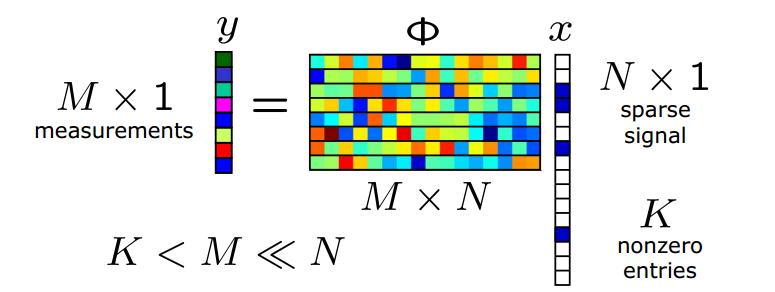
\includegraphics[height = 7 cm, width=\textwidth]{compressive_sensing_example.jpg}
\caption{A visualisation of the Compressive Sensing problem as an under-determined system}
\label{l1l2}
\end{figure*}

However, such and Oracle does not exist, and so we're left with the task of constructing a matrix to recover those components. Knowing that we're looking for k-sparse solutions, we need a matrix with at least 2k columns which are linearly independent. Equivalently, all images of \(k\)-sparse vectors under the operation of the sensing matrix \(\Phi\) must be distinct. From this, any k-sparse signal can be reconstructed from \(Ax\). 

To prove this assume the opposite - then there are two vectors \(x, x' \in \mathbb{R}^n\) such that \(Ax = Ax'\). I.e. \(A(x-x') = 0\). However, \((x-x')\) is 2k-sparse and so there is a linear dependence between 2k columns of the sensing matrix A. We have a contradiction, and so 2k columns will suffice to reconstruct a k-sparse signal. 

The problem with this is that we are trying to find the support of a k-sparse signal over a vector of length N, and so we would need to check all \(N \choose k\) combinations of k-sparse signals which is prohibitively computationally expensive. Is there some way to gain the advantages of sparsity, without having to minimise a non-convex functional?

As it turns out, the answer is yes. If we take \( m \geq C \mu^2(\phi, \psi) S \log\left(n\right) \) rows minimising the \(l_{1}\) norm will find the sparsest solution. This is because the \(l_1\) norm is an octahedron (in 3-dimensions, in higher dimensions it has an analogous spiky geometry), and solutions are more likely to intersect the norm at the points. Figure \ref{l1l2} shows this.

\begin{figure*}[h]
\centering
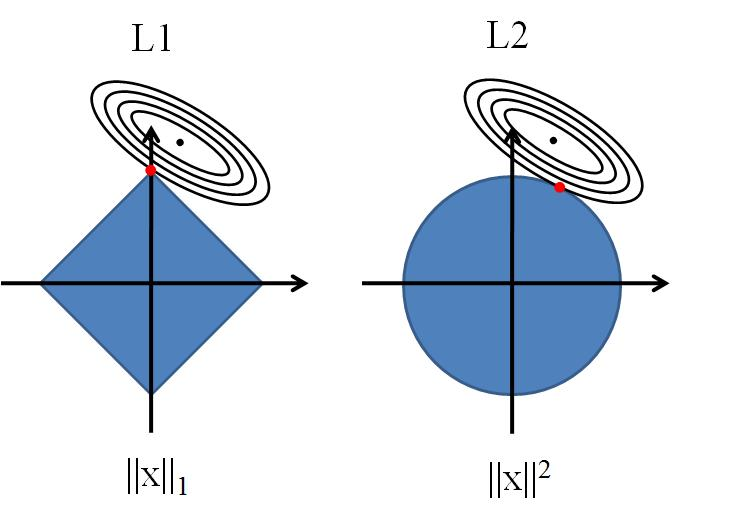
\includegraphics[height = 7 cm]{l1l2.jpg}
\caption{Solutions to the Compressive Sensing optimisation problem intersect the \(l_1\) norm the points where all components (but one) of the vector are zero (i.e. it is sparsity promoting) \cite{Tibshirani1996}}
\label{l1l2}
\end{figure*}

\subsubsection{Bayesian Compressive Sensing}
Based on the discussion above we can represent the compressive sensing measurements as: 

\begin{equation}
\textbf{g} = \Phi	\textbf{w}
\end{equation}

where \(\Phi\) is a \(K \times	N\) matrix which is the product of the measurement and sparse bases described earlier.

Note that the measurements may be noisy, with the measurement noise represented by a zero mean Gaussian distribution and unknown variance \( \sigma^2 \):

\begin{equation}
\textbf{g} = \Phi \textbf{w} + \textbf{n}
\end{equation}
\label{CSequation}

Where \textbf{n} is the vector representing the vector of noise, and has the same support as the measurements. 

Previous sections have shown how the weights \(w\) may be found through optimisation methods such as basis pursuit or greedy algorithms. Here, an alternative Bayesian model is described.

From \ref{CSequation} we have a Gaussian likelihood model: 

\begin{equation}
p \left( \textbf{g} \mid \textbf{w}\text{,} \sigma^2 \right) = (2 \pi \sigma^2)^{-K/2} \exp{\left(- \frac{1}{2 \sigma^2} \|\textbf{g} - \Phi	\textbf{w}\|_{2}^{2} \right)} 
\end{equation}

The above has converted the CS problem of inverting sparse weight \textbf{w} into a linear regression problem with a constraint (prior) that \textbf{w} is sparse. 

To seek the full posterior distribution over \textbf{w} and \( \sigma^2 \), we can chose a sparsity promoting prior. A popular sparseness prior is the Laplace density functions:

\begin{equation}
p\left(w\mid\lambda\right) = \left(\frac{\lambda}{2}\right)^N exp{-\lambda \sum_{i=1}^{N} |w_i|}
\end{equation}

Note that the solution the convex optimisation problem \ref{program0} corresponds to a maximum \textit{a posteriori} estimate for \(w\) using this prior. I.e this prior is equivalent to using the \(l_1\) norm as an optimisation function (see figure \ref{laplacenormal} \cite{Tibshirani1996}).

\begin{figure*}[h]
\centering
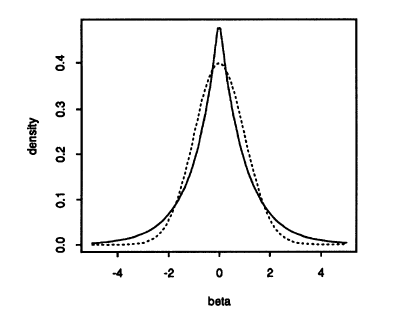
\includegraphics[height = 7 cm]{LaplaceandNormalDensity.png}
\caption{The Laplace (\(l_1\)-norm, bold line) and Normal (\(l_2\)-norm, dotted line) densities. Note that the Laplace density is sparsity promoting as it penalises solutions away from zero more than the Gaussian density. \cite{Tibshirani1996}}
\label{laplacenormal}
\end{figure*}

The full posterior distribution on \(w\) and \(\sigma^2\) may be realised, by using a hierarchical prior instead. To do this, define a zero-mean Gaussian prior on each element of \(w\):
%
\begin{equation}
p\left(w\mid a\right) = \prod_{i=1}^{N}\mathbb{N}\left(w_i\mid 0, \alpha_{i}^-1\right)
\end{equation}
%
where \(\alpha\) is the precision of the distribution. A gamma prior is then imposed on \(\alpha\):

\begin{equation}
p\left(\alpha \mid a, b \right) = \prod_{i=1}^{N} \Gamma\left( \alpha_i \mid a, b \right)
\end{equation}

The overall prior is found by marginalising over the hyperparameters:

\begin{equation}
p\left( w \mid a, b \right) = \prod_{i=1}^{N} \int_{0}^{\infty} \mathbb{N}\left(w_i\mid 0, \alpha_{i}^-1\right) \Gamma\left( \alpha_i \mid a, b \right)
\end{equation}

This integral can be done analytically and is a Student-t distribution. Choosing the parameters \(a,b\) appropriately we can make the Student-t distribution peak strongly around \(w_i = 0\) i.e. sparsifying. This process can be repeated for the noise variance \(\sigma^2\). The hierarchical model for this process is shown in \ref{bayesiancs}. This model, and other CS models which not necessarily have closed form solutions, can be solved via belief-propagation \cite{Baron2010}

\begin{figure*}[h]
\centering
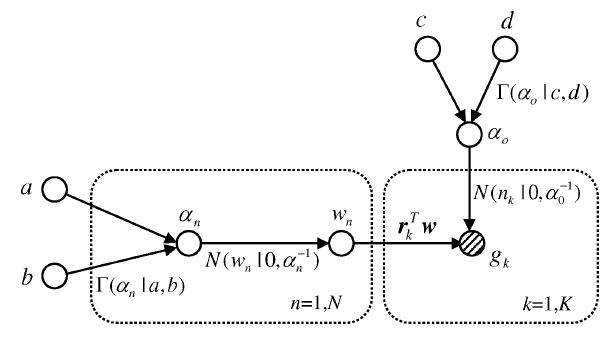
\includegraphics[height = 7 cm]{bayesiancs.png}
\caption{The hierarchical model for the Bayesian CS formulation \cite{Ji2008}}
\label{bayesiancs}
\end{figure*}


\subsection{Sub-Nyquist Sampling techniques}
This section presents some work on sampling methods for wide-band spectrum sensing

\subsubsection{Wideband Modulated Converter} 
The sampling scheme proposed in \cite{Mishali2010} is capable of sampling wideband signals at rates below those predicted by Shannon-Nyquist sampling theory. 

It works by mixing the incoming analogue signal \(x\left(t\right)\) with a mixing function \(p_i\left(t\right)\) aliasing the spectrum. \(x\left(t\right)\) is assumed to be bandlimited and composed of up to \(N_sig\) uncorrelated transmissions (i.e. possible narrowband channels). 

This process is repeated in parallel over \(M\) channels (unrelated to \(N_sig\) so that each band in \(x\) appears in baseband. The mixing functions are required to be periodic, with period \(T_p\). Since \(p_i\) is periodic it has Fourier expansion:

\begin{equation}
p_i\left(t\right) = \sum_{l=-\infty}^{\infty} c_{il} exp{jlt\frac{2\pi}{T_p}}
\end{equation}

The \(c_{il}\) are the Fourier coefficients of the expansion and are defined in the standard manner. The result of the mixing procedure in channel \(i\) is therefore \(xp_i\), with Fourier transform:

\begin{align}
X_{i}\left(f\right) &=& \int_{-\infty}^{\infty} x\left(t\right) p_i\left(t\right) dt
\\ &=& \sum_{l=-\infty}^{\infty} c_{il} X\left(f-lf_p\right)
\end{align}

\begin{figure*}[h]
\centering
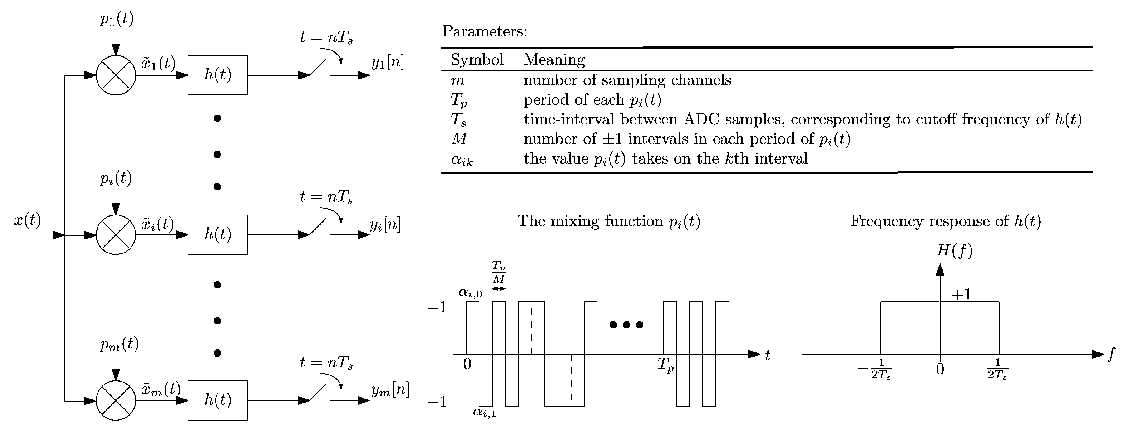
\includegraphics[height = 7 cm, width=\textwidth]{mwc.png}
\caption{The operation of the Modulated Wideband Converter \cite{mishali2010theory}}
\label{bayesiancs}
\end{figure*}

(insert the Fourier series for \(p_i\), then exchange the sum and integral). The output of this mixing process then, is a linear combination of shifted copies of \(X\left(f\right)\), with at most \(\lceil f_NYQ/f_p\rceil\) terms since \(X\left(f\right)\) is zero outside it's support (we have assumed this Nyquist frequency exists, even though we never sample at that rate).

Once the mixing process has been completed the signal in each channel is low-pass filtered and sampled at a rate \(f_s \geq f_p\). In the frequency domain this is a ideal rectangle function, so the output of a single channel is:

\begin{equation}
Y_i\left(e^{j 2 \pi f T_s }\right) = \sum_{l = -L_0}^{+L_0}
\end{equation}

since frequencies outside of \([-f_2/2, f_s/2]\) will filtered out. \(L_0\) is the smallest integer number of non-zero contributions in \(X\left(f\right)\) over \([-f_2/2, f_s/2]\) - at most \(\lceil f_NYQ/f_p\rceil\) if we choose \(f_s = f_p\). These relations can be written in matrix form as:

\begin{equation}
\textbf{y} = \textunderscore{\textbf{A}}\textbf{x}
\end{equation}

where \(\textbf{y}\) contains the output of the WMC process, \(\textunderscore{\textbf{A}}\) contains the Fourier coefficients of the mixing functions, and \(\textbf{x}\) is the vector of unknown samples of \(x\left(t\right)\). 

\section{Results and Simulations}
To compare the efficacy of Group Testing and Compressive Sensing, Hwang's algorithm and the algorithm presented in \cite{Aldrouobi} were simulated for a problem size of N=1024 and K=10.  The problem was simulated 100 times and the cumulative distribution found - i.e. after how many tests or measurements were the respective problems solved? This allows the number of tests required by Group Testing to be compared to the number of measurements in Compressive Sensing. Figure \ref{GTvsCS} shows the results:

\begin{figure*}[h]
\centering
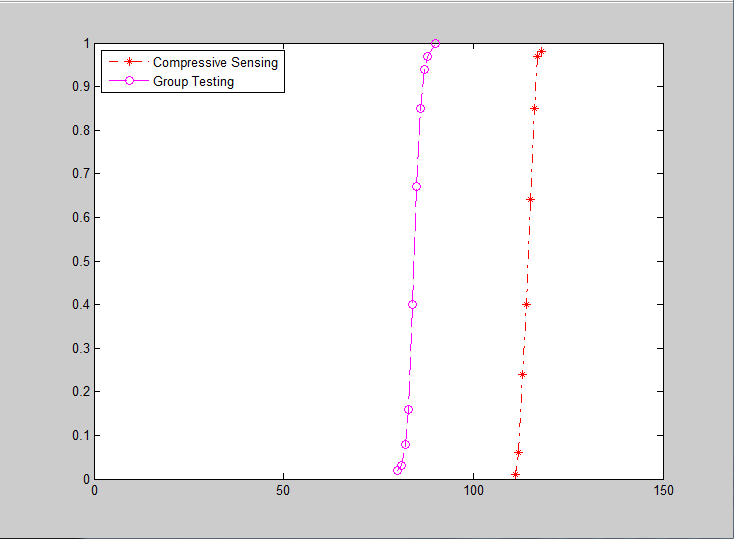
\includegraphics[height = 7 cm]{GTvsCS.png}
\caption{Group Testing vs Compressive Sensing}
\label{GTvsCS} 
\end{figure*}

Note that both the algorithms meet their respective asymptotic bounds (\( \log_2{N \choose K}\) in the case of GT and \(k\log{N}\) for CS). The main point of interest is that Group Testing requires roughly \(\frac{2}{3}\) of the tests required by Compressive Sensing. This is encouraging: despite there being 'less' information - in the sense that the result is a binary number as opposed to a real one -  GT outperforms CS. Intuitively, one would conjecture the opposite - more information should allow you to locate the non-zero components faster. This justifies our interest in the problem, as the performance increase is substantial. 

